\documentclass[11pt]{article}
\usepackage[letterpaper,margin=0.9in]{geometry}
\usepackage[T1]{fontenc}
\usepackage[utf8]{inputenc}
\usepackage{lmodern}
\usepackage{microtype}
\usepackage{parskip}
\usepackage{enumitem}
\usepackage{booktabs}
\usepackage{tabularx}
\usepackage{array}
\usepackage{hyperref}
\usepackage[round]{natbib}
\usepackage{xcolor}
\usepackage{fancyhdr}
\usepackage{amsmath,amssymb}
\usepackage{tikz}
\usetikzlibrary{arrows.meta,positioning,calc}
\setlength{\parindent}{0pt}
\setlength{\headheight}{14pt}
\hypersetup{colorlinks=true,linkcolor=black,citecolor=black,urlcolor=black}
\sloppy
\pagestyle{fancy}
\fancyhf{}
\lhead{\small The Vanishing Prompt}
\rhead{\small Question Paper}
\cfoot{\thepage}
\newcommand{\aph}[1]{\par\noindent\hangindent=2.0em\hangafter=1\makebox[1.6em][r]{\textbf{#1}\hspace{0.4em}}}

\begin{document}

\begin{center}
{\LARGE\bfseries The Vanishing Prompt}\\[0.35em]
{\large Operational Language and the Manufacture of Causal Certainty}\\[0.8em]
{\normalsize Watson Hartsoe}\\
{\small Question Paper --- 17 August 2026}
\end{center}

\vspace{0.4em}

\begin{abstract}
Prompt research is beginning to stabilize the prompt as a scientific object at the same moment that contemporary generative systems make that object increasingly difficult to locate. Recent work treats prompts as linguistic objects, structured discourse units, programs, and software-engineering artifacts; other work replaces discrete language with learned continuous prompts, rewrites or compiles instructions before execution, expands the operative input into dynamic context, demonstrates competition among explicit requirements, and shows that stochastic or temporal model state can materially determine generated artifacts. These findings do not merely add ``context'' to an otherwise stable prompt. They create an ontological problem. If a prompt is identified narrowly with the visible text, it is portable and versionable but causally incomplete. If it is enlarged until it contains the conditions that actually determine behavior, it expands toward the execution event and loses the bounded identity that made it a prompt. I call this the boundedness--causality dilemma. The consequence is methodological: prompt scholarship can manufacture causal certainty by treating the easiest thing to archive---the visible instruction---as the thing that caused the outcome. Drawing on recent prompt taxonomies, software-engineering accounts, soft prompting, context engineering, generative-model studies, and Suchman's critique of the planning model, this paper does not offer a replacement ontology. It asks a harder question: what kind of thing is a prompt if making it causally adequate makes it cease to be a prompt?
\end{abstract}

\noindent\textbf{Keywords:} prompts; operational language; prompt engineering; HCI; situated action; causal attribution; software engineering; generative AI

\vspace{0.6em}
\hrule
\vspace{0.3em}
\begin{flushright}
\scriptsize AI-augmented working paper. Research and assembly record accompanies the publication.
\end{flushright}

\section{The object arrives before its ontology}

Prompt researchers now have enough confidence in the word \emph{prompt} to build ontologies around it. In July 2026, Basmov, Goldberg, and Tsarfaty argued that prompts are ``linguistic objects'' worthy of scientific investigation, collected 57.5K transactional prompts from GitHub, and introduced an ontology for their formal and semantic components \citep{Basmov2026PromptsWild}. PromptPrism likewise analyzes prompts through functional, semantic, and syntactic structure and treats them as structured discourse units \citep{Jeoung2026PromptPrism}. Software-engineering researchers ask how prompts should be documented, traced, reused, and maintained as artifacts \citep{Villamizar2025PromptsArtifacts}; other work argues that some prompts are programs \citep{Liang2025PromptsPrograms}.

These projects solve real problems. They also expose an anomaly they cannot solve by adding another field to the taxonomy.

The prompt is easiest to stabilize precisely where its causal power is weakest: as stored text.

The text a researcher saves may not be the text a model receives. The effective control may not be text at all. The same string can behave differently when the system prompt, conversation state, retrieved material, model version, tokenizer, stochastic state, tools, decoding procedure, or selection rule changes. A concept can appear in an intermediate representation and disappear before the final artifact \citep{Agarwal2023ASTAR}. Initial diffusion noise can exhibit content preferences relative to a trained generator \citep{Mao2023InitialImageEditing}. Explicitly adding requirements can make other requirements less reliably followed \citep{Yang2025PromptsDontSay}. Continuous ``soft prompts'' can condition a frozen language model without being ordinary readable sentences \citep{Lester2021PromptTuning}.

The error is not that prompt scholars have ignored these complications. Many have documented them. The error is more basic: the field often continues to use \emph{prompt} as though all of those complications happened \emph{to one already-identifiable thing}.

That assumption has a cost. If the experimental unit is unstable, claims about prompt sensitivity can attribute an effect to wording that entered elsewhere. Prompt versioning can preserve a string while losing the conditions that made it operative. Reproducibility can become the reproduction of visible text rather than the reproduction of the event. Authorship can be assigned to language a user wrote even when a rewriter, compiler, learned vector, retrieval system, or optimizer supplied decisive control. A prompt history can look like the genealogy of a causal object when it is only the genealogy of one visible trace.

The problem is not that we know too little about prompts. It is that we may know many things about an object whose identity changes depending on what question we ask of it.

\section{The boundedness--causality dilemma}

A research object needs some condition under which we can say: \emph{this is the same object again}. Prompt research often obtains that identity cheaply. A prompt is the same prompt when its text, template, or structured message sequence is the same. That gives researchers something to save, diff, annotate, publish, version, and manipulate.

Call this the \emph{thin prompt}:

\[
P_{thin} = \text{the visible or stored instruction object}.
\]

The thin prompt is excellent archival material. It is often poor causal material.

A more causally serious account immediately begins to thicken it. The role-message structure matters. Hidden instructions matter. Retrieval matters. Prompt rewriting matters. Model version matters. Tokenization and representation matter. Tools matter. Random seed or sampling state may matter. Candidate selection matters. For a deployed system, one might write only schematically:

\[
Y = S\big(G_{\theta}(E(R(P),C,T),Z)\big),
\]

where \(P\) is visible text; \(R\) is any rewrite or assembly process; \(C\) is contextual material; \(T\) represents tools or schemas; \(E\) is model-relative representation; \(Z\) is stochastic state; \(G_{\theta}\) is model execution under parameters \(\theta\); and \(S\) is any downstream selection. This is not source syntax. It is a pressure test on the noun \emph{prompt}.

Every time an external variable proves behaviorally consequential, there are two choices.

First, keep it outside the prompt. The prompt remains bounded, but a growing share of the cause lies elsewhere.

Second, absorb it into the prompt. The prompt becomes more causally adequate, but less like the object the field began with.

\begin{figure}[ht]
\centering
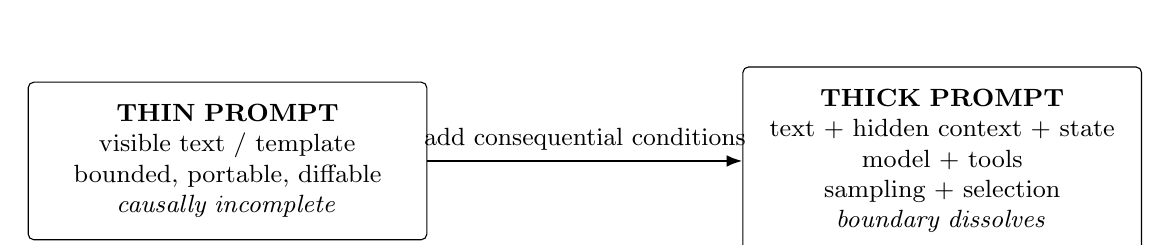
\begin{tikzpicture}[
box/.style={draw,rounded corners=2pt,inner sep=8pt,align=center,font=\small,text width=4.5cm,minimum height=1.35cm},
arr/.style={-{Latex[length=2mm]},thick}
]
\node[box] (thin) {\textbf{THIN PROMPT}\\visible text / template\\bounded, portable, diffable\\\emph{causally incomplete}};
\node[box, right=4.0cm of thin] (thick) {\textbf{THICK PROMPT}\\text + hidden context + state\\model + tools\\sampling + selection\\\emph{boundary dissolves}};
\draw[arr] (thin.east) -- node[above,font=\small]{add consequential conditions} (thick.west);
\end{tikzpicture}
\caption{The boundedness--causality dilemma. A conceptual pressure test, not a claim that all systems share one pipeline.}
\label{fig:dilemma}
\end{figure}

Context engineering already concedes the first half of this problem. Mei et al. argue that contemporary systems do not operate on one static string and explicitly replace the historical equation \(C=\text{prompt}\) with a dynamically assembled set of contextual components \citep{Mei2025ContextEngineering}. That is an important correction. Yet it does not dissolve the ontology problem. It relocates it. Once ``context'' includes retrieval, memory, multimodal material, state, tool-integrated reasoning, and orchestration, the research object has moved from an instruction toward a system-level execution condition. The box becomes more accurate by becoming larger.

The question cannot be settled by announcing that the prompt is ``really context.'' The same regress begins again: which parts of context count as the operative object, and which remain conditions of its use?

This is why the prompt is both something and almost nothing. It is something because inscriptions matter: change a word and behavior can change. It is almost nothing because the inscription never carries its operative force alone. The same sentence is not the same intervention when the machinery that receives it changes.

\section{HCI has seen this mistake before}

The prompt problem has an older shape.

Suchman's \emph{Plans and Situated Actions} attacked a planning model that treated plans as though they determined situated conduct. Her point was not that plans are useless. Plans are consequential resources. The mistake is to substitute the plan for the action whose course is contingently produced in a situation \citep{Suchman1987Plans}. Retrospectively, action can be made to look as though it simply realized the plan. The mess by which the action actually came to be disappears.

Prompt scholarship risks rebuilding this mistake inside HCI and software engineering.

A prompt resembles a plan in the dangerous respect. It is available before action, legible afterward, and easy to place next to the result. The pairing invites a reconstruction: the model did \(Y\) because the prompt said \(X\). Hidden instructions, model priors, state, retrieval, stochastic trajectories, and selection become implementation detail. The visible instruction acquires explanatory privilege because it survives the event as text.

That privilege is not absurd. A prompt can be an effective resource for action. Suchman's argument makes the stronger causal reading harder, not the weaker practical one. The question is whether a prompt determines, specifies, or reconstructs execution---and whether researchers notice when they slide among those verbs.

The analogy also exposes why ``better prompt documentation'' cannot by itself solve the problem. A perfectly archived plan is still not an archive of the situated action. A perfectly archived prompt can still omit the state in which its operative significance was produced.

HCI may already possess the conceptual warning prompt research now needs: the representational object available to the analyst is not automatically the unit that organized the event.

\section{The word \emph{prompt} fractures under use}

The literature now contains several objects called prompts that do not share one obvious ontology.

\subsection{The linguistic object}

Basmov et al. ground part of their ontology in what they call inherent prompt properties: prompts are texts written in a language, formulate a task, and serve to elicit output \citep{Basmov2026PromptsWild}. PromptPrism likewise obtains analytic power by decomposing prompt discourse into structural, semantic, and syntactic dimensions \citep{Jeoung2026PromptPrism}. This is valuable if the object of study is \emph{prompt language}: the inscriptions developers place in software, their forms, distributions, tasks, and rhetorical structures.

The problem begins when linguistic identity silently becomes operational identity.

A text can be classified without establishing that the same classification identifies the relevant cause of downstream behavior. A system message and user message can be separated as discourse roles while both are still only portions of an executed context. A template can be recovered from source code while runtime values, retrieval results, tools, state, and model behavior remain elsewhere. The ontology answers ``what is in this text?'' more securely than ``what was the operative object in this run?''

These are different questions. The first does not deserve criticism for failing to answer the second. The trouble is the ease with which a phrase such as ``prompts directly shape behavior'' lets one answer inherit the authority of the other.

\subsection{The software artifact}

Software engineering wants a more durable object. Villamizar et al. propose treating prompts as potential software-engineering artifacts and study their evolution, traceability, reuse, documentation, and management \citep{Villamizar2025PromptsArtifacts}. The move is practical: systems need maintainable objects.

Yet their borrowed definition of an artifact is revealing. An artifact is a self-contained work result with representation, syntax, and semantics. Prompted systems are interesting precisely because the effective instruction is frequently not self-contained. The same text can change meaning when inserted into a different hierarchy of messages, model, context, tool schema, or interaction history.

The software-engineering need for a stable artifact and the empirical instability of the operative object pull in opposite directions.

Version control makes the tension visible. If version \(P_1\) and version \(P_2\) are two strings, a diff is exact. If a provider changes the model behind the same API, the prompt file can remain byte-identical while behavior changes. If retrieval changes, the committed template remains identical while the instantiated context does not. If an optimizer compiles a new executed prompt, the developer's source declaration can remain stable while the instruction presented to the model changes \citep{Khattab2023DSPy}.

What, then, evolved?

The artifact framing is not wrong. It is caught between two kinds of identity: identity for maintenance and identity for causal explanation.

\subsection{The nonlinguistic prompt}

Soft prompting makes the contradiction sharper. Lester, Al-Rfou, and Constant learn continuous vectors through backpropagation to condition frozen language models \citep{Lester2021PromptTuning}. Qin and Eisner likewise describe ``soft words'' that need not correspond to ordinary word embeddings \citep{QinEisner2021SoftPrompts}.

A field can respond in two ways.

It can say that these are not really prompts because they are not language. That saves the linguistic ontology by excluding a technical tradition already named prompt tuning.

Or it can admit them as prompts. Then textuality is not an inherent property of prompts after all.

Neither choice is trivial. The term has become useful across the boundary that its ontology would need to draw.

This is one reason the prompt feels vaporous. It persists as a name while the substance beneath the name changes: sentence, template, role-message bundle, learned vector, prefix, generated instruction, dynamic context component. The family resemblance is functional---something conditions what the model will do---but that functional definition is so broad that model weights, retrieved documents, tools, and random state begin to knock at the door.

\subsection{The specification that loses force when specified}

Yang et al. show that LLMs sometimes satisfy requirements absent from the written prompt, but those unstated behaviors are fragile across model or prompt changes; they also show that adding more explicit requirements does not reliably improve instruction following because constraints can compete \citep{Yang2025PromptsDontSay}.

This result unsettles the everyday metaphor of the prompt as specification. If specifying a requirement can reduce effective control, then the quantity of specification in the text and the quantity of constraint on behavior are not monotonically related.

The missing requirement is not simply missing from the system. It may be supplied by model priors. The written requirement is not simply present in behavior. It may be ignored, displaced, or interfere with another instruction. The operative ``specification'' is distributed across inscription and machinery.

A prompt can be more explicit and less determinative.

\subsection{The instruction that enters time}

Image generation makes visible something text-only prompt accounts easily hide: instructions have careers inside execution.

A-STAR reports compositional failures in diffusion generation where concept-specific attention may appear early yet fail to persist through later denoising \citep{Agarwal2023ASTAR}. Mao et al. show that regions of initial latent noise can have reproducible content preferences relative to a trained diffusion model \citep{Mao2023InitialImageEditing}. Simonen et al. find recurring ``default images'' from dissimilar prompts and show that seed, model version, and recognized prompt terms alter the phenomenon \citep{Simonen2026DefaultImages}.

These studies make ``the prompt caused the image'' radically underspecified. Did the requested concept never enter the representation? Did it enter and decay? Did a recognized neighbor dominate it? Did the initial state make one recurrent motif easier to realize? Did a hidden transformation alter the input before denoising began?

The final image cannot answer those questions. Neither can the original sentence.

\section{How causal certainty gets manufactured}

The prompt interface presents a seductive diagram: text on one side, output on the other. Scholarship can inherit the diagram without noticing.

A researcher changes a phrase and records a performance difference. The phrase becomes the intervention. A paper reports a ``prompt effect.'' The result may be completely real. What remains underdetermined is the locus of the effect.

The certainty is manufactured in four quiet moves.

\textbf{First, observability becomes ontology.} The string is the thing we can recover from code, show in an appendix, annotate, and place in a dataset. Its visibility makes it feel like the natural unit.

\textbf{Second, temporal adjacency becomes causal privilege.} The user writes, then the model responds. Intermediate transformations and states are hidden, so the visible predecessor receives explanatory credit.

\textbf{Third, successful reconstruction erases situated production.} Once an output looks responsive, we read the prompt backward through it: of course the model did this because the prompt said that. The output supplies coherence to the instruction after the fact.

\textbf{Fourth, reproducibility is reduced to inscription.} We save the prompt and call the experiment reproducible even when model version, hidden context, rewrite policy, retrieval corpus, stochastic state, or evaluator is unavailable.

None of these moves requires bad science. They arise from ordinary experimental necessity. Researchers need variables. Engineers need artifacts. Datasets need rows. Reviewers need methods that can be inspected. The prompt is an extraordinarily convenient handle.

The handle becomes a culprit only when convenience hardens into causal ontology.

This is why merely expanding metadata is insufficient. More metadata can improve reproducibility enormously, but the ontological problem is not missing columns. It is deciding which columns belong to the object and which belong to the situation in which the object acts. If every consequential condition is pulled inside the prompt, the prompt eventually becomes indistinguishable from the execution record.

The problem has the shape of a whirlpool: to explain the prompt's force we add its context; to explain the context we add the mechanism that assembled it; to explain the mechanism we add model and state; to explain the result we add selection. Each addition makes the account better and the original noun thinner.

At some point explanation has not clarified the prompt. It has made it disappear.

\section{Remarks toward a missing ontology}

The following remarks do not resolve the problem. They are attempts to keep its edges from being smoothed away.

\aph{1.} A prompt is easiest to identify before execution and hardest to identify after it has worked.

\aph{2.} The text survives. The conditions that made it an instruction do not.

\aph{3.} Two saved strings can be identical while their acts are not.

\aph{4.} Two different strings can become the same instruction after a rewriter has finished with them.

\aph{5.} A soft prompt is called a prompt at the point where language has vanished.

\aph{6.} We keep the noun by changing what the noun names.

\aph{7.} The instruction that is absent from the text may still be present in the model.

\aph{8.} The instruction that is present in the text may never become present in the artifact.

\aph{9.} More specification can produce less obedience. A specification is not measured by how much has been said.

\aph{10.} The seed is called random because of how it is sampled, not because all its futures are equivalent inside a trained generator.

\aph{11.} When a concept appears early and disappears later, ``the model ignored the prompt'' confuses a history with an outcome.

\aph{12.} We save the sentence and call the experiment reproducible.

\aph{13.} The experiment is sometimes reproducible only at the level of typography.

\aph{14.} The prompt is not nothing. If it were nothing, changing it would do nothing.

\aph{15.} The prompt is not the whole thing. If it were the whole thing, keeping it fixed would keep the act fixed.

\aph{16.} To make the prompt causally adequate, we enlarge it until it is no longer a prompt.

\aph{17.} A taxonomy can tell us what is written without telling us what acted.

\aph{18.} A version history can preserve every sentence and lose the event.

\aph{19.} ``The model followed the prompt'' is often a retrospective description of correspondence, not a located mechanism.

\aph{20.} The prompt is the name we give to the part of the cause we can see.

\section{The harder questions}

A missing ontology should not be repaired by choosing a better slogan. ``Prompt,'' ``context,'' ``program,'' ``artifact,'' and ``execution lineage'' each stabilize a different slice of the phenomenon. The useful question is what evidence would force us to distinguish them.

\begin{enumerate}[leftmargin=1.6em]
\item \textbf{What are the identity conditions of a prompt?} If the text is identical but the model, system message, retrieved context, or tool schema changes, is it the same prompt? If the text changes but an upstream compiler maps both forms to the same executed representation, are they different prompts?

\item \textbf{Which prompt properties are intrinsic and which are relational?} Language, syntax, and visible role structure can be properties of an inscription. ``Effective instruction,'' ``constraint,'' ``meaning,'' and ``control'' may exist only in relation to a particular model and runtime.

\item \textbf{Where does prompt meaning happen?} Is meaning adequately located in the visible discourse, in tokenizer and embedding geometry, in activation patterns, in an evolving generation trajectory, or only in the relation between the request and a selected outcome?

\item \textbf{What survives transplantation?} Move the identical prompt across model versions, vendors, system messages, tools, languages, seeds, and context assemblers. Which properties remain invariant enough to justify saying it is one operational object?

\item \textbf{What is reproduced when we reproduce a prompt?} A string, an instruction, an experimental condition, a probability distribution over behaviors, or a historical interaction?

\item \textbf{When should ``prompt'' be retired from a causal claim?} A paper may still study prompt texts linguistically while refusing to treat them as sufficient causal units. What vocabulary marks that boundary without replacing one false totality with another?

\item \textbf{Can the field distinguish prompt efficacy from prompt attribution?} An edit can improve performance even when the reason it works is not where the editor thinks it is. Does successful control require correct causal understanding?

\item \textbf{Who authored the operative instruction?} The user, developer, system-prompt author, retriever, compiler, model provider, optimizer, evaluator, or the interaction among them?

\item \textbf{What is the negative space of a prompt?} Which behavior is supplied by model defaults, training histories, safety layers, or conventions precisely because it was not written?

\item \textbf{What evidence could show that the prompt really is the right unit?} The burden should run both ways. If there are domains in which visible text interventions remain causally stable under controlled runtime variation, those are boundaries worth finding.
\end{enumerate}

These questions alter what counts as a useful experiment. The aim is no longer simply to discover which wording ``works.'' It is to locate invariants and discontinuities across layers of execution. One can hold visible text constant while varying runtime conditions; hold transformed input constant while varying surface wording; preserve model and context while varying stochastic state; inspect whether requested semantics enter and survive internal trajectories; compare candidate distributions before selection. Each intervention asks not merely \emph{whether} prompts matter, but \emph{in what sense the thing called a prompt remains the same while they matter}.

\section{Boundary}

The argument here should not be inflated into the claim that prompt texts are epiphenomenal. They plainly matter in many systems. Nor does the existence of hidden variables invalidate studies that deliberately choose linguistic prompts as their object. Basmov et al. explicitly focus on transactional prompts recoverable from particular software APIs and state that their ontology is extensible rather than exhaustive \citep{Basmov2026PromptsWild}. PromptPrism makes a linguistic taxonomy and demonstrates uses for linguistic analysis \citep{Jeoung2026PromptPrism}. Those projects can remain valuable without carrying the additional burden of an ontology of situated execution.

The problem appears when a bounded textual object is asked to do more than the evidence permits: to stand simultaneously as linguistic artifact, program, specification, experimental treatment, reproducible condition, unit of authorship, and causal explanation.

Those roles may coincide in some systems and diverge in others. The divergence is the research territory.

Nor does ``context engineering'' solve the problem simply by adopting a wider scope. Its recognition that modern systems operate on dynamic, structured information streams is crucial \citep{Mei2025ContextEngineering}. Yet a larger context variable can become another convenient container whose boundaries are fixed by engineering practice rather than causal identity. The challenge is not finding the largest noun.

It is learning when to stop pretending that a noun has stayed the same.

\section*{Coda}

The prompt began as a box one could type into.

Research made the box into a method, then an artifact, then a program, then a language, then an ontology.

The machinery beneath the box kept moving.

Perhaps \emph{prompt} will survive as a modest name for a visible inscription used to intervene in a generative system. That would be enough. A handle need not be the whole machine.

What should not survive is the convenience by which the handle impersonates the cause.

\vspace{0.8em}
\begin{center}
\emph{The prompt is the name we give to the part of the cause we can see.}
\end{center}

\begin{thebibliography}{99}
\bibitem[Agarwal et~al.(2023)Agarwal, Karanam, Joseph, Saxena, Goswami, and Srinivasan]{Agarwal2023ASTAR}
Aishwarya Agarwal, Srikrishna Karanam, K.~J. Joseph, Apoorv Saxena, Koustava Goswami, and Balaji Vasan Srinivasan. 2023.
\newblock A-STAR: Test-time attention segregation and retention for text-to-image synthesis.
\newblock In \emph{Proceedings of ICCV 2023}, 2283--2293.

\bibitem[Basmov et~al.(2026)Basmov, Goldberg, and Tsarfaty]{Basmov2026PromptsWild}
Victoria Basmov, Yoav Goldberg, and Reut Tsarfaty. 2026.
\newblock Prompts in the Wild: A Large Analyzed Collection of Transactional Prompts in Code.
\newblock In \emph{Proceedings of the 20th Linguistic Annotation Workshop (LAW XX)}, 257--308. Association for Computational Linguistics. doi:10.18653/v1/2026.law-main.19.

\bibitem[Jeoung et~al.(2026)Jeoung, Chen, Zhang, Wang, Ding, and Cheong]{Jeoung2026PromptPrism}
Sullam Jeoung, Yueyan Chen, Yi Zhang, Shuai Wang, Haibo Ding, and Lin Lee Cheong. 2026.
\newblock PromptPrism: A Linguistically-Inspired Taxonomy for Prompts.
\newblock In \emph{Findings of the Association for Computational Linguistics: EACL 2026}, 1168--1192. doi:10.18653/v1/2026.findings-eacl.61.

\bibitem[Khattab et~al.(2023)Khattab et~al.]{Khattab2023DSPy}
Omar Khattab, Arnav Singhvi, Paridhi Maheshwari, Zhiyuan Zhang, Keshav Santhanam, Sri Vardhamanan, Saiful Haq, Ashutosh Sharma, Thomas T. Joshi, Hanna Moazam, Heather Miller, Matei Zaharia, and Christopher Potts. 2023.
\newblock DSPy: Compiling Declarative Language Model Calls into Self-Improving Pipelines.
\newblock arXiv:2310.03714.

\bibitem[Lester et~al.(2021)Lester, Al-Rfou, and Constant]{Lester2021PromptTuning}
Brian Lester, Rami Al-Rfou, and Noah Constant. 2021.
\newblock The Power of Scale for Parameter-Efficient Prompt Tuning.
\newblock In \emph{Proceedings of EMNLP 2021}.

\bibitem[Liang et~al.(2025)Liang, Lin, Rao, and Myers]{Liang2025PromptsPrograms}
Jenny T. Liang, Melissa Lin, Nikitha Rao, and Brad A. Myers. 2025.
\newblock Prompts Are Programs Too! Understanding How Developers Build Software Containing Prompts.
\newblock \emph{Proceedings of the ACM on Software Engineering}, 2. doi:10.1145/3729342.

\bibitem[Mao et~al.(2023)Mao, Wang, and Aizawa]{Mao2023InitialImageEditing}
Jiafeng Mao, Xueting Wang, and Kiyoharu Aizawa. 2023.
\newblock Guided Image Synthesis via Initial Image Editing in Diffusion Model.
\newblock arXiv:2305.03382.

\bibitem[Mei et~al.(2025)Mei et~al.]{Mei2025ContextEngineering}
Lingrui Mei, Jiayu Yao, Yuyao Ge, Yiwei Wang, Baolong Bi, Yujun Cai, Jiazhi Liu, Mingyu Li, Zhong-Zhi Li, Duzhen Zhang, Chenlin Zhou, Jiayi Mao, Tianze Xia, Jiafeng Guo, and Shenghua Liu. 2025.
\newblock A Survey of Context Engineering for Large Language Models.
\newblock arXiv:2507.13334.

\bibitem[Qin and Eisner(2021)]{QinEisner2021SoftPrompts}
Guanghui Qin and Jason Eisner. 2021.
\newblock Learning How to Ask: Querying LMs with Mixtures of Soft Prompts.
\newblock arXiv:2104.06599.

\bibitem[Simonen et~al.(2026)Simonen, Kiviniemi, Johnston, Barranha, and Oppenlaender]{Simonen2026DefaultImages}
Hannu Simonen, Atte Kiviniemi, Hannah Johnston, Helena Barranha, and Jonas Oppenlaender. 2026.
\newblock An Exploration of Default Images in Text-to-Image Generation.
\newblock In \emph{Proceedings of CHI 2026}. doi:10.1145/3772318.3790681.

\bibitem[Suchman(1987)]{Suchman1987Plans}
Lucy A. Suchman. 1987.
\newblock \emph{Plans and Situated Actions: The Problem of Human-Machine Communication}.
\newblock Cambridge University Press.

\bibitem[Villamizar et~al.(2025)Villamizar, Fischbach, Korn, Vogelsang, and Mendez]{Villamizar2025PromptsArtifacts}
Hugo Villamizar, Jannik Fischbach, Alexander Korn, Andreas Vogelsang, and Daniel Mendez. 2025.
\newblock Prompts as Software Engineering Artifacts: A Research Agenda and Preliminary Findings.
\newblock arXiv:2509.17548.

\bibitem[Yang et~al.(2025)Yang, Shi, Ma, Liu, K\"astner, and Wu]{Yang2025PromptsDontSay}
Chenyang Yang, Yike Shi, Qianou Ma, Michael Xieyang Liu, Christian K\"astner, and Tongshuang Wu. 2025.
\newblock What Prompts Don't Say: Understanding and Managing Underspecification in LLM Prompts.
\newblock arXiv:2505.13360.
\end{thebibliography}

\appendix
\section{Assembly and provenance note}
This manuscript is a working paper assembled from a preserved research field and then rebuilt after an explicit tension-first and ontology-first critique. The central revision did not treat the prior paper's ``execution lineage'' or ``causal attribution'' theses as inherited conclusions. It re-opened the field around the unstable identity of the prompt itself. A claim-source map, Axis Inversion report, philosophical diagnostic, deep-question register, and newly foraged zettels accompany this PDF in the publication package.

\end{document}
